\documentclass[12pt]{article}

\usepackage{amsfonts}
\usepackage{amsthm}
\usepackage{amsmath}
\usepackage{amssymb}
\usepackage{mathtools}
\usepackage{xcolor}
\usepackage[normalem]{ulem}
\usepackage{hyperref}
\hypersetup{
    colorlinks=true,
    linkcolor=blue
}


\newcommand{\floor}[1]{\lfloor #1 \rfloor}
\newcommand{\FF}{\mathbb{F}}
\newcommand{\ZZ}{\mathbb{Z}}
\newcommand{\LL}{\mathcal{L}}
\DeclareMathOperator{\Span}{Span}


\newtheorem{question}{Question}
\newtheorem{lemma}{Lemma}
\newtheorem{theorem}{Theorem}
\newtheorem{remark}{Remark}
\newtheorem{definition}{Definition}



\title{Comparing Lattice Families for Bounded Distance Decoding near Minkowski’s Bound}

\author{ Oleksandra Lapiha }
\usepackage{xcolor}
\def\added{\bgroup \markoverwith{\textcolor{green!50!blue}{\lower4.5pt\hbox{\sixly \char58}}}\ULon}
\def\toimprove{\bgroup \markoverwith{\textcolor{red}{\lower4.5pt\hbox{\sixly \char58}}}\ULon}
\def\improved{\bgroup \markoverwith{\textcolor{black}{\lower4.5pt\hbox{\sixly \char58}}}\ULon}


\begin{document}

\maketitle

\section{Introduction}
\label{sec:intro}
\textbf{Bounded Distance Decoding problem.} Message decoding is a problem that arises when two parties need to communicate over a noisy channel. Here we are in the setting where we are only concerned with the integrity of transmitted data and we assume there's no adversary listening and modifying messages in the network. We are dealing with information loss that occurs due to our information flow being \textit{slightly disturbed} by forces of nature.

To achieve that we encode messages as points in Euclidean space. Now we can model the rate of "disturbance" as distance between the input and output points. And call it "slight" if it can be bounded by a constant. A natural way to arrange the space of messages is a Euclidean lattice(all integer linear combinations of a linearly independent set of vectors in $\mathbb{R}^{n}$).

The decoding procedure aims to identify the point of the lattice closest to the output point. If the disturbance in the network is small enough the closest lattice point will indeed be the input message. This will help us identify the upper bound on how much error a perfect decoding algorithm can handle. We know that the distance between lattice points is bounded from below by the length of the shortest vector($\lambda_{1}(\LL)$) of the lattice. If the error exceeds $\frac{\lambda_{1}(\LL)}{2}$, the closest point might not be the input message anymore so decoding becomes impossible.

We would like to have an algorithm where the decoding radius is close to $\frac{\lambda_{1}(\LL)}{2}$. Unfortunately, the Lattice Shortest Vector Problem(SVP) is believed to be hard in the general case, so we cannot evaluate exactly how good our decoding radius is. Nevertheless, we have an upper-bound on the length of the shortest vector. So we aim to get a decoding radius close to it instead.
\begin{theorem}[Minkowski's First Theorem]
    For any full-rank lattice $\LL$ of rank $n$,
    \[
        \lambda_{1}(\LL) \leq \sqrt{n} \det(\LL)^{1/n}
    \]
\end{theorem}

An instance of such problem is called a Bounded Distance Decoding problem and it is considered a hard problem for a random lattice and decoding radius of $\frac{\lambda_{1}(\LL)}{2}$ in the norm $l_{\infty}$ \cite{[LM09]}.


Our work focuses on two families of lattices for which BDD problem has an efficient solution and error is close to the Minkowski's bound. The first one is a generalization of a lattice discussed in \cite{[DP19]} and used in Chor-Rivest cryptosystem \cite{[CR88]}. The second one was used in \cite{[LLXY17]} for construction of a trapdoor function and has a similar decoding algorithm. Apart from decoding algorithms we discuss an efficient way to compute the basis of a given lattice. It is important to be able to compute some representation of the lattice efficiently because this is a way to craft lattice points from messages we would like to transmit.

In this work we generalize the lattice family from \cite{[DP19]} and suggest an efficient way to compute it. The decoding algorithm of the same article extends to our case directly. The second lattice family was discussed in \cite{[LLXY17]} we extend the decoding algorithm devised for them to handle more types of error. We also suggest security improvements for the encryption scheme from \cite{[LLXY17]} using our decoding algorithm and perform its cryptanalysis to improve their parameter selection.


\textbf{Discrete logarithm lattices.}
In this work we will discuss many lattices of similar flavour. They are defined as a kernel of a morphism from $\ZZ^{n}$ to another group. Let us give you a short definition of the lattice given in \cite{[DP19]} which serves as a basis for our first generalization.

Let us consider numbers $m$ which is a prime power, $n$ and $B$ such that we can find $n$ primes $p_{1}, \dots , p_{n}$ which do not divide $m$ and are bounded by $B$. We consider a group morphism:
\[
    \psi : \ZZ^{n} \rightarrow (\ZZ/m\ZZ)^*
\]
\[
    (x_{1}, \dots, x_{n}) \mapsto \prod_{i=1}^{n}p_{i}^{x_{i}} \pmod{m}
\]
It is easy to see that the image will indeed be an element of $(\ZZ/m\ZZ)^*$ due to our parameter selection. The kernel of $\psi$ is a subgroup of $\ZZ^{n}$ so it is a lattice.
\[
    \LL \coloneqq \ker \psi = \{(x_{1}, \dots, x_{n}) \in \ZZ^{n} | \prod_{i=1}^{n}p_{i}^{x_{i}} \equiv 1 \pmod{m}\}
\]

The basis of this lattice is simple to compute it only requires computation of $n$ discrete logarithms in $(\ZZ/m\ZZ)^*$ it can be done because the multiplicative group of a field $\ZZ/m\ZZ$ is cyclic. Discrete logarithms can be computed in polynomial time as they are calculated modulo a smooth number. More on that you can find in \cite{[DP19]}. The generalization we give will require more work in this regard.

\textbf{Efficient decoding algorithm.}

We use a decoding algorithm discussed in \cite{[DP19]} and \cite{[LLXY17]}. We provide a few modifications for it to fit our scenario in the second part of the work, but the skeleton of the algorithm will stay the same. We are given a lattice $\LL$ defined above and a point $t = (t_1, \dots t_n) \in \mathbb{R}^{n}$ which doesn't belong to $\LL$ and we would like to find the lattice point $x$ closest to $t$. We assume that error is a vector of real numbers whose norm is bounded. The algorithm has the following building blocks:

\begin{itemize}
    \item Round every coordinate to $t$ to deal only with discrete error $\lfloor t \rceil = x + \lfloor e \rceil$. Note $e' = \lfloor e \rceil$, $t' = \lfloor t \rceil$. Lattice point $x$ is not affected by this operation since $\LL \subset \ZZ^{n}$.
    \item Compute $\psi(t) = \prod_{i=1}^{n}p_{i}^{x_{i} + e'_i} \pmod{m} = \prod_{i=1}^{n}p_{i}^{e'_i} \pmod{m}$. If the error is small enough here we recover non-reduced value $v = \prod_{i=1}^{n}p_{i}^{e'_i}$.
    \item Reconstruct the numerator $n$ and the denominator $d$ of $v$ that correspond to positive and negative parts of the error. Recover prime number factorization of $n$ and $d$ using trial division. Powers of primes will be the coordinates of our error.
    \item Subtract just recovered error from $t'$.
\end{itemize}


In this work by an efficient algorithm we mean an algorithm that runs in polynomial time.

\textbf{Organisation of the document.}
In the section \ref{sec:gen_integers} we discuss the first lattice family. We detail on:
\begin{itemize}
    \item how to compute its basis \ref{subsec:compute_basis_integers}
    \item what it the complexity of this algorithm \ref{subsec:complexity_integers}
    \item and how much of the error we can decode \ref{subsec:radius_integers}
\end{itemize}
The next part of our work \ref{sec:polynomials} is dedicated to the family of polynomial lattices.
\begin{itemize}
    \item it's basis computation is discussed in the section \ref{subsec:compute_basis_polynomials}
    \item the decoding radius for this case is discussed in \ref{subsec:radius_polynomials}
    \item \textcolor{red}{ToDo:} maybe rename sections so they follow the same pattern in the second part.
\end{itemize}
Then we compare these two families with respect to basis computation and decoding algorithms in \ref{sec:comparison}. Finally, we perform cryptanalysis of the encryption scheme presented in \cite{[LLXY17]} and propose improvements to it in the section \ref{sec:cryptanalysis}.

\textbf{Implementation.}
Sagemath implementation of every algorithm for basis computation and message decoding discussed in the document is available on github via link: \textcolor{red}{TBA}.

\section{Generalization of the construction for integers}
\label{sec:gen_integers}
In this section we present a generalization of the decoding algorithm introduced in \cite{[DP19]}. In their paper Léo Ducas and Cécile Pierrot use properties of the group $(\ZZ/m\ZZ)^*$ for modulus $m$ which is a prime power. The decoding radius achievable in polynomial-time depends on the ratio
\[
\frac{\ln(m)}{\varphi(m)}
\]
The higher the ratio the larger the achievable decoding radius will be. In our generalization we take $m'$ an arbitrary product of prime powers. If $m$ and $m'$ are of the same size, as $m'$ is smoother $\varphi(m')$ will be smaller which gives us a better decoding radius.

In the construction for $m$ prime power authors compute lattice basis directly using the fact that $(\ZZ/m\ZZ)^*$ is cyclic and we can calculate discrete logarithms of its elements.

Our result is a deterministic efficient algorithm for computation of the basis for any integer $m$. We find a way to deal with the structure of the group $(\ZZ/m\ZZ)^*$ in a different way and compute lattice basis through its dual.


\subsection{Definition of discrete logarithm lattice }
\label{subsec:def_integers}
In this chapter we take $m = \prod_{i=1}^{k} q_{j}^{e_{j}}$ where $\{q_{j}\}$ are odd prime numbers and $\{e_{j}\}$ are positive integers. Similarly to the initial construction we take numbers $n$ and $B$ such that we can find $n$ primes $p_{1}, \dots , p_{n}$ different from every $q_{j}$ and bounded by $B$. We consider a group morphism:
\[
    \psi : \ZZ^{n} \rightarrow (\ZZ/m\ZZ)^*
\]
\[
    (x_{1}, \dots, x_{n}) \mapsto \prod_{i=1}^{n}p_{i}^{x_{i}} \pmod{m}\footnote{Since  $p_{1}, \dots , p_{n}$ are relatively prime with $m$ for every element of $\ZZ^{n}$ its image is indeed a part of $ (\ZZ/m\ZZ)^*$.}
\]


The kernel of $\psi$ is a subgroup of $\ZZ^{n}$ so it is a lattice. We will call it discrete logarithm lattice from now on.
\[
    \LL \coloneqq \ker \psi = \{(x_{1}, \dots, x_{n}) \in \ZZ^{n} | \prod_{i=1}^{n}p_{i}^{x_{i}} \equiv 1 \pmod{m}\}
\]

We work with a group $(\ZZ/m\ZZ)^*$ which is not cyclic anymore so we cannot exploit properties of discrete logarithm right away. Nevertheless, the Chinese Remainder Theorem (CRT) gives us the structure of the group:
\[
   (\ZZ/m\ZZ)^* \sim \prod_{j=1}^{k}(\ZZ/q_{j}^{e_{j}}\ZZ)^*
\]
For every prime $q_{j} > 2$ and every $e_{j} \geq 1$ the group $(\ZZ/q_{j}^{e_{j}}\ZZ)^*$ is known to be cyclic. So now, we can consider discrete logarithms in every component of the product to find a lattice basis.

Applying the CRT gives us the following equivalence
\[
    \LL = \ker \psi = \{(x_{1}, \dots, x_{n}) \in \ZZ^{n} |  \forall 1 \leq j \leq k: \prod_{i=1}^{n}p_{i}^{x_{i}} \equiv 1 \pmod{q_{j}^{e_{j}}}\}
\]
Going even further, suppose we know for every $j$ a generator ${\beta_{j}}$ of  $(\ZZ/q_{j}^{e_{j}}\ZZ)^*$. Using the morphism between the cyclic group and group of exponents we get a representation in terms of conditions on the exponents:
\[
    \LL = \{(x_{1}, \dots, x_{n}) \in \ZZ^{n} |  \forall 1 \leq j \leq k: \sum_{i=1}^{n}x_{i}\log_{\beta_{j}}p_{i}\equiv 0 \pmod{\varphi(q_{j}^{e_{j}})}\}
\]
Note that discrete logarithm functions that we are using have different input and output domains
\[
    \forall 1 \leq j \leq k: \log_{\beta_{j}}: (\ZZ/q_{j}^{e_{j}}\ZZ)^* \rightarrow (\ZZ/\varphi(q_{j}^{e_{j}})\ZZ)
\]
This is almost a parity check representation of $\LL$ except we have many parity check type conditions at the same time. Therefore, $\LL$ is an intersection of lattices $\LL_{j}$ where each of them is defined as
\[
\label{parity check}
    \LL_{j} \coloneqq \{(x_{1}, \dots, x_{n}) \in \ZZ^{n} | \sum_{i=1}^{n}x_{i}\log_{\beta_{j}}p_{i}\equiv 0 \pmod{\varphi(q_{j}^{e_{j}})}\}
\]

\subsection{Computing lattice basis}
\label{subsec:compute_basis_integers}
Our goal is to compute a basis of discrete logarithm lattice to be able to encode messages as its points afterwards. The idea of our algorithm is to compute a basis of the dual lattice first. And then obtain primal one from the dual.
Let us recall a definition of a dual lattice and a dual basis.
\begin{definition}
    For a lattice $\LL \subseteq \mathbb{R}^{n}$ we define $\LL^{*} \subseteq (\mathbb{R}^{n})^{*}$ as a lattice of all linear maps $f:\mathbb{R}^{n} \rightarrow \mathbb{R}$ such that every lattice point is mapped to an integer value.
\end{definition}
Linear maps can be represented as an inner product function with a fixed vector. So equivalently
\[
    \LL^{*} = \{y \in \mathbb{R}^{n} | \forall x \in \LL:  \langle x,y\rangle \in \ZZ \}
\]

\begin{definition}
    For a basis $B = (b_{1}, \dots, b_{n}) \in \mathbb{R}^{m \times n}$, define the dual basis $D = (d_{1}, \dots, d_{n}) \in \mathbb{R}^{m \times n}$ as the unique basis that satisfies
    \begin{itemize}
        \item $\Span(D) = \Span(B)$
        \item $B^{T}D = I$
    \end{itemize}
\end{definition}
If B is a square matrix then $(B^{T})^{-1}$ satisfies the definition. In the case of a non square matrix one can verify that $D = B(B^{T}B)^{-1}$ is the dual basis. \footnote{Since columns of $B$ are basis vectors, $B$ is a full column rank matrix. Therefore, $B^{T}B$ is always invertible.}


 Our algorithm \label{algorithm} has the following steps
\begin{enumerate}
    \item \label{step1} Calculate parity check representations for every $\LL_{j}$
    \item \label{step2} Get dual generating set of their intersection
    \item \label{step3} Eliminate linear dependencies in the generating set
    \item \label{step4} Obtain the basis of the primal lattice from the dual
\end{enumerate}
We will describe each of them in more details

\subsubsection{Parity check representations (\ref{step1})}
\label{subsubsec:parity_check_repr}
In the section \ref{subsec:def_integers} we were able to represent $\LL$ as an intersection of $\LL_{1}, \dots, \LL_{k}$ for which we have parity check representations:
\[
    \LL_{j} \coloneqq \{(x_{1}, \dots, x_{n}) \in \ZZ^{n} | \sum_{i=1}^{n}x_{i}\log_{\beta_{j}}p_{i}\equiv 0 \pmod{\varphi(q_{j}^{e_{j}})}\}
\]
To compute them we calculate many discrete logarithms in finite groups. As you probably know it is a hard problem for a general case of which no polynomial algorithm is known. We need to choose parameters such that we can compute them efficiently. We discuss it in the section (\ref{subsec:complexity_integers}) of this document.

\subsubsection{Dual generating set (\ref{step2})}
\label{subsubsec:dual_gen_set}
To justify this step we need two lemmas
\begin{definition}
    For two lattices $\LL_1$, $\LL_2$ we define their sum
\[
    \LL_1 + \LL_2 \coloneqq \{x + y | x \in \LL_1, y \in \LL_2\}
\]
\end{definition}
This space $\LL_{1} + \LL_{2}$ can be generated by concatenation of bases of $\LL_{1}$ and $\LL_{2}$. It is a sum of two additive subgroups of $\mathbb{R}^{n}$ so it stays an additive subgroup. But it is not always discreet so it doesn't necessarily form a lattice.

\begin{lemma}
    \footnote{Check it again with fresh head}
    \label{lemma_intersection}
    Suppose $\LL = \bigcap_{j=1}^{k} \LL_{j} \neq \{0\}$ and $\LL^{*}$, $\LL_{j}^{*}$ are duals of the respective lattices. Then $\LL^{*} = \sum_{j=1}^{k} \LL_{j}^{*}$
\end{lemma}
\begin{proof}
    Let us start from the end. Take lattices $\LL_{1}, \dots, \LL_{n}$ which is the dual of their sum.
    \footnote{We can take all $x_{i}$ equal to 0 but 1 of them}
\[
\begin{split}
(\sum_{j=1}^{n}\LL_j)^{*} & = \{y \in \ZZ^{n} | \forall x_{1} \in \LL_1, \dots, \forall x_{n} \in \LL_n: \langle y, \sum_{j=1}^{n} x_{j} \rangle \in \ZZ \} \\
& = \{y \in \ZZ^{n} | \forall 1 \leq j \leq n, \forall x_{j} \in \LL_j: \langle y,  x_{j} \rangle \in \ZZ \}
\end{split}
\]

So $y$ must be an element of every $\LL_{j}^{*}$. Therefore, $(\sum_{j=1}^{n}\LL_j)^{*} = \bigcap_{j=1}^{k} \LL_{j}^{*}$. Applying this assertion to lattices $\LL_{1}^{*}, \dots, \LL_{n}^{*}$ we have
\[
(\sum_{j=1}^{n}\LL_j^{*})^{*} = \bigcap_{j=1}^{k} \LL_{j} = \LL
\]
Now taking dual lattices of both sides of the equation we obtain:
\[
(\sum_{j=1}^{n}\LL_j^{*})^{**} = \LL^{*}
\]

\end{proof}

\begin{lemma}
    Let B be a square matrix, $B \in \mathbb{R}^{n \times n}$. Suppose we are given parity check representation of a lattice $\LL = \{x \in \ZZ^{n} | Bx \equiv 0 \pmod{p}\}$
    Then \textbf{rows} of the matrix
    \[
    \binom{\frac{1}{p} \cdot B}{I_{n}}
    \]
    form a generating set of the dual lattice.
\end{lemma}
\begin{proof}
    Another equivalent definition for $\LL$ would be:
    \[
        \LL  = \{x \in \ZZ^{n} | \frac{1}{p}Bx \equiv 0 \pmod{1}\}
    \]
Therefore, can represent $\LL$ as an intersection of the following lattices:
\[
    \LL_{1}  = \ZZ^{n}
\]
\[
    \LL_{2}  = \{x \in \mathbb{R}^{n} | \frac{1}{p}Bx \in \ZZ^{n} \}
\]
Then from lemma \ref{lemma_intersection}
\[
    \LL^{*}  = (\LL_{1} \cap \LL_{2})^{*} = \LL_{1}^{*} + \LL_{2}^{*}
\]
It is obvious that $(\ZZ^{n})^{*} = \ZZ^{n}$. To prove that $(\frac{1}{p}B)^{T}$(here basis vectors are columns) is a basis of the dual it is enough to show $(\frac{1}{p}B)^{-1}$ is basis of the primal lattice. This is quite simple:
\[
    \forall x \in \ZZ^{n}: \frac{1}{p}B \cdot (\frac{1}{p}B)^{-1} \cdot x \in \ZZ
\]
And the other way:
\[
    \forall x \in \LL: \frac{1}{p}B \cdot x = y \in \ZZ^{n} \implies x = (\frac{1}{p}B)^{-1} \cdot y , y \in \ZZ^{n}
\]
A generating set of the sum of lattices can be obtained by concatenation of their bases, so we obtain our desired result.
\end{proof}

The basis computation algorithm takes parity check representations of every lattice $\LL_{j}$ scales them and adds an identity matrix. Output is the concatenation of calculated generating sets.

\subsubsection{Eliminating linear dependencies using elementary matrix transformations (\ref{step3})}
\label{subsubsec:hermite_form}
Now we have obtained a generating set of the dual lattice but we would like to have its basis. The idea is to transform the matrix to its row echelon form so the resulting set has some zero vectors which we will discard and obtain the basis of the lattice.

Out of all elementary matrix transformations we are only allowed adding to a row an integer multiple of another row, interchanging two rows, multiplying a row by -1. These three possibilities are called unimodular transformations. As you may have noticed the only restriction is that we can't multiply a row by an integer different from $\pm 1$. This would result in a sublattice of $\LL$ with a higher determinant.

We use an algorithm for reducing the matrix to its Hermite normal form. It is an equivalent of row echelon form for matrices over $\ZZ$ with a restriction to unimodular transformations. Our input matrix can have rational coefficients so we first transform them into integers multiplying by the least common multiple of all denominators. We divide by it when the matrix is in the Hermite form.

Resulting vectors might be quite long. If we want to control the size of the basis we can use the LLL algorithm instead. This change will for example make our encoded messages shorter and easier to decode.

\subsubsection{Primal basis from dual basis (\ref{step4})}
\label{subsubsec:primal_from_dual}
A way to calculate a basis of primal lattice having the basis of the dual is straightforward having its definition.


\subsection{Complexity analysis}
\label{subsec:complexity_integers}
The first step (\ref{step1}) of the basis computation algorithm (\ref{algorithm}) boils down to many computations of discrete logarithms in a finite group. For every distinct prime factor $q_{j}^{e_{j}}$ of the modulus we compute $n$ discrete logarithms(one for every prime $p_{i}$). It is $n \cdot k$ iterations in total. Let's refer to $(\ZZ/q_{j}^{e_{j}}\ZZ)^*$ as group $G$. Group order is equal to $|G| = \varphi(q_{j}^{e_{j}}) =  q_{j}^{e_{j}-1}(q_{j}-1) = \prod_{i=1}^{k} t_{i}^{a_{i}}$.
It is a $q$-smooth integer, so to efficiently calculate discrete logarithms in this group we can use a combination of of Pohlig-Hellman \cite{[PH78]} and Pollard-$\rho$ \cite{[Pol78]} algorithms. Overall complexity in group operations is
\[
    O(\sum_{i=1}^{k} a_{i}(\ln(|G|) + \sqrt{t_{i}}))
\]
To be polynomial in lattice dimension $a_{i} \leq e_{j}-1$ and $t_{i} \leq q_{j}$ need to be polynomial in $n$. As we have $n \cdot k$ such operations, $k$ should be polynomial in $n$.

It is easy to see that step two (\ref{step2}) takes linear time in $n + k$. Step three (\ref{step3}) is Hermite normal form reduction which has the same complexity as Gaussian elimination so runs in time polynomial in $n + k$.

Finally, step four (\ref{step4}) includes matrix multiplication and inversion for matrices whose dimension is bounded by $n + k$. They take polynomial time.



\subsection{Decoding radius}
\label{subsec:radius_integers}

Decoding algorithm extends naturally to the generalized setting. Let us remind that normalized decoding $l_{1}$-radius was equal to
\[
    \bar r_{1} = \frac{\ln(m/2)}{4 \varphi(m)^{1/n} \cdot \ln(B)}
\]
where $B$ is a constant bounding all $p_{i}$

We still haven't configured parameters $k, q_{j}, p_{i}$. $q_{j}, p_{i}$ must be pairwise different and as small as possible, so we need $n+k$ distinct prime numbers. We choose $p_{i}$ to be equal to first $n$ prime numbers and $q_{j}$ equal to the next $k$ smallest primes that we haven't used yet.

The ratio $\frac{ln(m/2)}{\varphi(m)}$ decreases as $m$ tends to infinity, so to make use of the difference in the ratio in the generalization, we would like $m$ to have the same size as in the original construction. We would like to have $e_i \sim \frac{\ln(3) \cdot n}{\ln(q) \cdot k}$, but it has to be an integer, so we round this value. Then we have:
\[
    m = \prod_{i = 1}^{k} q_i^{round(\frac{\ln(3) \cdot n}{\ln(q) \cdot k})} \sim 3^n
\]

The only parameter left to configure is $k$. The way we set up $e_i$s number of factors will only increase the ratio $\frac{ln(m/2)}{\varphi(m)}$. So the more factors we have the better.

Let us compare initial construction, its generalization and theoretical upper bound with respect to the decoding radius.

\begin{figure}
  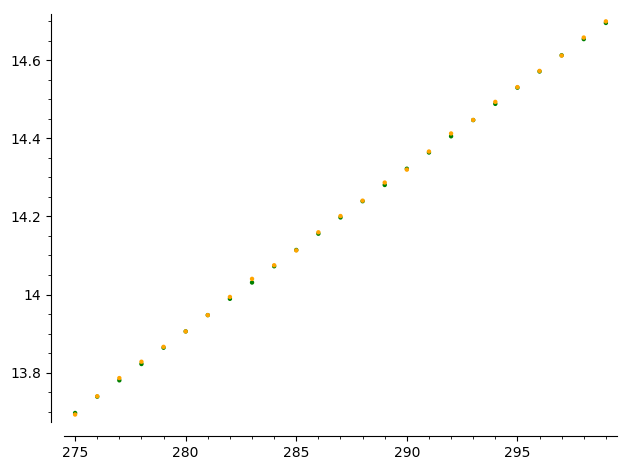
\includegraphics[width=\linewidth]{generalization_integers.png}
  \caption{Comparison of the normalised decoding radius for initial construction(in green) and the generalization(in yellow). Here we took k = 20. }
  \label{fig:gen_int}
\end{figure}

\subsection{Was it all worth it?}
\label{subsec:improvement_integers}
As it turns out factorization of $m$ does not affect the decoding radius substantially. It can only introduce a minor improvement. We prove that with the following lemma:

\begin{lemma}
Assume the primes $p_{1}, \dots, p_{n}$ are the same for both lattices. If $a \cdot m \sim b \cdot m' \sim e^n$, when $n \rightarrow \infty$ Then
\[
    \frac{\bar r_{m}^{(1)}}{\bar r_{m'}^{(1)}} \rightarrow 1, n \rightarrow \infty
\]
\end{lemma}
\begin{proof}
Since the primes are the same, they are also bounded by the same constant $B$ so the term $\frac{1}{4 \ln(B)}$ cancels out in the numerator and denominator.
\[
\begin{split}
\frac{\bar r_{m}^{(1)}}{\bar r_{m'}^{(1)}}
& = \frac{\ln(m/2) \cdot \varphi(m')^{1/n}}{\ln(m'/2) \cdot \varphi(m)^{1/n}} \\
& = \frac{\ln(e^n/2a) \cdot \varphi(m')^{1/n}}{\ln(e^n/2b) \cdot \varphi(m)^{1/n}} \\
& = \frac{\varphi(m')^{1/n}}{\varphi(m)^{1/n}}
\end{split}
\]
We apply a few classic results to estimate the growth of $\varphi(n)$ \cite{[HW09]}:
\[
    \limsup\limits_{n \rightarrow \infty} \frac{\varphi(n)}{n} = 1
\]
\[
    \liminf\limits_{n \rightarrow \infty} \frac{\varphi(n) \cdot \ln\ln(n)}{n} = e^{-\gamma}
\]
where $\gamma$ is the Euler constant, $e^{-\gamma} = 0.56145948\dots$
\[
\begin{split}
\lim_{n \rightarrow \infty} \frac{\varphi(m')^{1/n}}{\varphi(m)^{1/n}}
& \leq \frac{\limsup\limits_{n \rightarrow \infty} \varphi(m')^{1/n}}{\liminf\limits_{n \rightarrow\infty}\varphi(m)^{1/n}} \\
& = \lim_{n \rightarrow \infty} \bigg(\frac{m \cdot \ln\ln (m')}{m'}\bigg)^{1/n} \\
& = \lim_{n \rightarrow \infty} (\ln\ln(e^n/b))^{1/n} = 1
\end{split}
\]
\end{proof}



\section{New Construction for Polynomial Lattices}
\label{sec:polynomials}
\subsection{Definition of Polynomial Lattices}
\label{subsec:def_polynomials}
Let us set parameters a prime power $q$ and integers $k$, $d$ and $n$. Let $\FF_{q}[x]$ be polynomial ring over a field  $\FF_{q}$. We take a set of $k$ irreducible polynomials $c_{j}(x) \in \FF_{q}[x]$, $j =1, ...,k$ of degree $d$. According to the analogue of the prime number theorem for polynomials $k$ must not be greater than $\frac{q^d}{d}$.

Define $c(x) \coloneqq \prod_{j = 1}^{k} c_{j}(x)$. We are going to work in the multiplicative group of the quotient ring of  $\FF_{q}[x]$ with respect to $c(x)$.
Chinese Remainder Theorem helps to determine the structure of $\big(\FF_{q}[x]/c(x)\big)^{*}$:
\[
    \big(\FF_{q}[x]/c(x)\big)^{*} \sim \prod_{i=1}^{k}\big(\FF_{q}[x]/c_{i}(x)\big)^{*} \sim \prod_{i=1}^{k}\FF_{q^{d}}^*
\]
Multiplicative group of a field is cyclic, therefore, we can consider discrete logarithms in every component of the product to find a lattice basis.

Consider a vector $a = (\alpha_{1}, ... , \alpha_{n}) \in \FF_{q}^{n}$ where $\alpha_{i}$s are pairwise different. Since polynomials $c_{j}(\cdot)$ are irreducible over $\FF_{q}$ neither of $\alpha_{i}$ can be their root. So for all $\alpha_{i}$ we also have: $c(\alpha_{i}) \neq 0$.

Now consider a group morphism:
\[
    \psi : \ZZ^{n} \rightarrow \big(\FF_{q}[x]/c(x)\big)^{*}
\]
\[
    (u_{1}, ..., u_{n}) \mapsto \prod_{i=1}^{n}(x - \alpha_{i})^{u_{i}} \pmod{c(x)}
\]

Lattice is defined as the kernel of the morphism:
\[
    \LL = \ker \psi = \{(u_{1}, ..., u_{n}) \in \ZZ^{n} | \prod_{i=1}^{n}(x - \alpha_{i})^{u_{i}} \equiv 1 \pmod{c(x)}\}
\]
Applying CRT gives us the following equivalence
\[
    \LL = \ker \psi = \{(u_{1}, ..., u_{n}) \in \ZZ^{n} |  \forall 1 \leq j \leq k: \prod_{i=1}^{n}(x - \alpha_{i})^{u_{i}} \equiv 1 \pmod{c_{j}(x)}\}
\]
Supposing we know $\beta_{j}$ a generator of $\big(\FF_{q}[x]/c_{j}(x)\big)^{*}$ for every $j$ we get another representation:
\[
    \LL = \{(u_{1}, ..., u_{n}) \in \ZZ^{n} | \forall 1 \leq j \leq k: \sum_{i=1}^{n}u_{i}log_{\beta_{j}}(x - \alpha_{i}) \equiv 0 \pmod{q^{d} -1}\}
\]
What might be confusing is that each $\log_{\beta_{j}}$ has a different input domain. For every $j$:  $\log_{\beta_{j}}$ acts from $\big(\FF_{q}[x]/c_{j}(x)\big)^{*}$ into $(\ZZ/(q^{d} - 1)\ZZ)$.

We obtained a parity check representation of $\LL$.
To calculate a basis of $\LL$ we can follow simplified version of the algorithm for integers. We obtain dual basis by scaling parity check matrix and concatenating it with $I_{n}$. Then we remove linear dependencies and finally obtain primal basis from the dual.

\subsection{Lattice computation for polynomials}
\label{subsec:compute_basis_polynomials}

\subsubsection{Factorization by trial division}
\label{subsubsec:factoring_polynomials}
Input: A polynomial $g$ such that $deg(g) \leq m$ whose roots are among $\alpha_1, \dots , \alpha_n \in \mathbb{F}_q$\\
Output: $e_1, \dots , e_n$ s.t. $g = \prod_{i = 1}^{n}(x - \alpha_i)^{e_i}$\\
There's only $n$ possible roots, one trial division takes $O(m)$ time and the number of factors is bounded by $m$. So overall complexity is $O(m^2n)$.


\subsubsection{Rational function reconstruction}
\label{subsubsec:rfr}
I found \href{http://www.cecm.sfu.ca/~mmonagan/papers/fastRFR.pdf}{here}
an algorithm which they call Wang's algorithm for rational function reconstruction.\\
Goal: Given $g,f$ find $n, d \in \mathbb{F}[x]$ that $deg(n) + deg(d) < \frac{deg(f)}{2}$ and $\frac{n}{d} = g \pmod{f}$\\
Algorithm:(function $lc()$ outputs the leading coefficient)
\begin{enumerate}
    \item   $r_0 = f$  $r_1 = g$\\
            $t_0 = 0$  $t_1 = 1$\\
            $q = 1$\\
    \item While $deg(q) \leq \frac{deg(f)}{2}$ do\\
            $q = r_0 // r_1$\\
            $(r_0, r_1) = (r_1, r_0 - qr_1)$\\
            $(t_0, t_1) = (t_1, t_0 - qt_1)$\\
    \item if $GCD(r_0, t_0) \neq 1$ or $deg(r_0) + deg(t_0) \geq \frac{deg(f)}{2}$:\\
            return FAIL\\
          else:\\
            return $(\frac{r_0}{lc(t_0)}, \frac{t_0}{lc(t_0)})$
\end{enumerate}
\begin{lemma}
Let $\mathbb{F}$ be a field, $f, g, r, s, t \in \mathbb{F}[x]$ with $r = sf + tg$, $t \neq 0$, $deg(f) > 0$, and $deg(r) + deg(t) <deg(f)$.
Suppose $r_i, s_i, t_i$ for $0 \leq i \leq l + 1$ be the elements of the ith iteration in the Extended Euclidean Algorithm for $f$ and $g$ (e.i. $r_i = s_if + t_ig$). \\
Then there exists a nonzero element $\alpha \in \mathbb{F}[x]$ such that $r = \alpha r_j$, $s = \alpha s_j$, $t = \alpha t_j$, where $deg(r_j) \leq deg(r) < deg(r_{j-1})$
\end{lemma}
\begin{proof}
\href{http://www.cecm.sfu.ca/~mmonagan/theses/sara.pdf}{(Lemma 3.2 page 35)}
\end{proof}

So if the solution exists it must be one of the pairs $(r_i, t_i)$ of the EEA.

\textcolor{red}{ToDo:} Add a lemma to prove the following: If $deg(n) + deg(d) \leq \frac{deg(f)}{2}$ than the solution corresponds to the unique row of the EEA where $deg(q) > \frac{deg(f)}{2}$

\begin{question}
Check if we can use FEEA.
\end{question}
\subsubsection{Computing logs}
\label{subsubsec:logs_polynomials}
To construct the lattice we need to compute the following:
$\forall 1 \leq i,j \leq n :$ $log_{\beta_j}(x - \alpha_i) \pmod{q^{d} -1}$. The order of multiplicative group is $q^{d} - 1$ which might not be a smooth integer so we cannot use Pohlig-Hellman+Pollard pho. We can choose $q^{d} = n^{O(1)}$ ($poly(n)$) so group order is overall small(e.g. $d = constant$ and $q=n^{O(1)}$ does work, so does $q=constant$ and $d = O(\log n)$).

\subsubsection{Recovering Primal basis from Dual}
\label{subsubsec:primal_from_dual_polynomials}


\subsection{Complexity of the basis computation.}
\label{subsec:complexity_polynomials}
Let us analyse every step of the basis computation algorithm to check if it is efficient:
\begin{itemize}
    \item
    \item
\end{itemize}


\subsection{Decoding radius}
\label{subsec:radius_polynomials}

\subsubsection{Only positive discrete error}
\label{subsubsec:positive_error}
Suppose we receive $t = u + e$ where $u \in \mathcal{L}$, $\|e\|_1 \leq r_1$ and $\forall i: e_i \in \mathbb{N}$. Then we can compute
\[
\prod_{i = 1}^{n}(x - \alpha_i)^{t_i} = \prod_{i = 1}^{n}(x - \alpha_i)^{u_i}\prod_{i = 1}^{n}(x - \alpha_i)^{e_i} \pmod{c(x)}
\]
If $\|e\|_1 = \sum_{i =1}^{n} e_i \leq deg(c) = d \cdot k$ the operation above will give us exactly the polynomial $\prod_{i = 1}^{n}(x - \alpha_i)^{e_i}$. Then we can recover $e_i$, $1 \leq i \leq n$ from the factorization.\\
So $l_1(r_1) = d \cdot k$.

Due to the nature of the bound above it is natural to talk about the length $r_1$ in $l_1$ norm.
\subsubsection{Arbitrary discrete error}
\label{subsubsec:discrete_error}
Now we have $\forall i: e_i \in \mathbb{Z}$. Then
\[
\prod_{i = 1}^{n}(x - \alpha_i)^{t_i} \pmod{c(x)} = \prod_{i = 1}^{n}(x - \alpha_i)^{e_i} = \frac{\prod_{i \in I}(x - \alpha_i)^{e_i}}{\prod_{j \in J}(x - \alpha_j)^{-e_j}}
\]
\begin{lemma}
Given $g,c$ where $deg(c) = d \cdot k$ we can recover $f_{1}, f_{2} \in \mathbb{F}[x]$ that  $\forall i = 1;2$: $deg(f_{i}) \leq \floor{\frac{dk}{2}}$ and $\frac{f_{1}}{f_{2}} = g \pmod{c}$ in polynomial time.
\end{lemma}
So we can decode every message for which $\|e\|_1 = \sum_{i =1}^{n} |e_i| \leq \floor{\frac{dk}{2}}$
\subsubsection{Normalized radius}
\label{subsubsec:normalized_discrete_error}
Directly follows from \cite{[DP19]}. $\bar{r}_1 = \frac{dk}{det(\mathcal{L})^{1/n}}$ where $det(\mathcal{L}) = \Phi(c(x)) = (q^{d} - 1)^{k}$.
\[
\bar{r}_1 = \frac{dk}{(q^{d} - 1)^{k/n}}
\]
What should be the values of $d$ and $k$?

We have the following constraints:
\begin{enumerate}\label{constraints}
    \item $q^d = n^{O(1)}$
    \item $dk < q^{d}$
    \item $n \leq q$
\end{enumerate}
From these we can immediately conclude that $d$ must be constant \\

We aim to be at most a logarithmic factor away from Minkowski bound, for that this asymptotics suffice: $q = a \cdot n$, $d = b$, $k =  c \cdot \frac{n}{\log(n)}$. What we are going to do next is finding optimal values for parameters $a, b$ and $c$. We want to maximize the following function:
\[
\bar{r}_1 = \frac{bc \cdot n}{\log(n)((an)^{b} - 1)^{c/\log(n)}}  \sim \frac{bc \cdot n}{e^{bc}\log(n)}
\]
 Parameter $a$ by constraint 3 in \ref{constraints} should be greater or equal to 1.
 \[
    \frac{bc \cdot n}{\log(n)((an)^{b} - 1)^{c/\log(n)}} \leq \frac{bc \cdot n}{\log(n)(n^{b} - 1)^{c/\log(n)}}
 \]

The choice of $a$ does not affect choices of $b$ and $c$ so we can configure it to 1.

The function we are considering with fixed parameters $c, b$ tend to the same value as $\frac{bc \cdot n}{\log(n)n^{cb/\log(n)}}$. To simplify the analysis we will find the best parameters for the latter.

Note $d \coloneqq bc$, $f_n(d) = \frac{d \cdot n^{1 - \frac{d}
{\log(n)} }}{\log(n)}$.
We would like to prove that for any value of $n$, $argmax(f_n(d)) = 1$
\[
\begin{split}
    f_n'(d) & = \frac{n^{1 - \frac{d}
    {\log(n)}}}{\log(n)} + \frac{d \cdot n^{1 - \frac{d}
    {\log(n)}} \cdot \log(n) \big(-\frac{1}{\log(n)}\big)}{\log(n)} \\
    & = \frac{n^{1 - \frac{d}{\log(n)}}}{\log(n)}(1-d)
\end{split}
\]
$d = 1$ is the only solution to the equation $f_n'(d) = 0$. It is easy to verify that it corresponds to the maximum of $f_n(d)$ and it doesn't depend on the value of $n$.

Therefore, $b \cdot c = 1$. In practice we fix $b = 2, c = \frac{1}{2}$. In the end, the decoding radius our algorithm achieves is
\[
    \bar{r}_1 = \frac{n}{\log(n)(n^{2} - 1)^{1/2\log(n)}}
\]

\subsection{Comparing the decoding radius of the algorithms}
\label{sec:comparison}

For the first family final normalized error radius that the algorithm can handle is:
\[
    \bar{r}_1 = \frac{\ln(m/2)}{4 \cdot \varphi(m)^{1/n} \cdot \ln((n+1)\ln(n+1))}
\]
And for the second construction it is much better:
\[
    \bar{r}_1 = \frac{n}{\log(n)(n^{2} - 1)^{1/2\log(n)}}
\]
But both of them are still logatihmically far from Minkowski's bound. The figure \ref{fig:everything} will help you to see the difference in practice.

\begin{figure}
  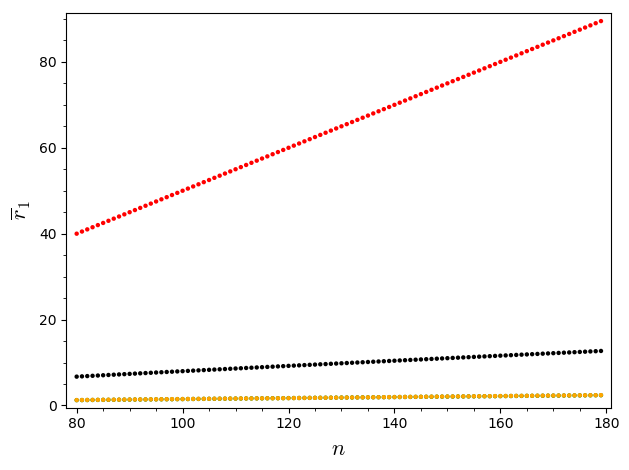
\includegraphics[width=\linewidth]{everything.png}
  \caption{Comparison of all algorithms and theoretical upperbound(in red): basic algorithm for integer lattice(in green), generalized algorithm for integer lattice(in yellow), algorithm for polynomial lattices(in blue)}
  \label{fig:everything}
\end{figure}

\section{LLXY17 Cryptanalysis?}
\label{sec:cryptanalysis}

\subsection{Classic attacks on lattices}
\label{subsec:attacks}

\subsubsection{ISD Attack}
\label{subsec:isd_attack}

\subsubsection{MitM Attack}
\label{subsec:mitm_attack}

\subsubsection{ISD+MitM Combination}
\label{subsec:combination_attack}

\subsection{Improving LLXY17 parameter selection}
\label{subsec:param_improvement}

\subsection{Adding negative errors}
\label{subsec:negative_error_improvement}
Our algorithm allows to decode negative errors efficiently, so adding it will improve security. By how much?

\bibliography{report}
\bibliographystyle{ieeetr}

\end{document}
